\section{Introducing \acs{NMR}}

\subsection{A Brief History of NMR}
The origins of \ac{NMR} can be traced back to 1945, when independent work by
Felix Bloch on water\cite{Bloch1946} and Edward Purcell on
parrafin\cite{Purcell1946} gave rise to the first illustrations of nuclear
magnetic resonances in condensed phases. The two hadn't met before their
respective papers were published with about a month's
separation\cite{Becker1993}. Both received the Nobel Prize in Physics in 1952
for their pioneering work in the field. A notable mention should also be given
to Yevgeny Zavoisky, the father of Electron Paramagnetic Resonance, who
probably observed NMR as far back as 1941\cite{Eaton1998}. Alas, he dismissed
his results as irreproducible. In 1949 and 1950, work investigating \ac{NMR}
spectra from compounds containing Cu, \textsuperscript{31}P,
\textsuperscript{14}N, and \textsuperscript{19}F nuclei illustrated the concept
of the chemical shift\cite{Knight1949, Proctor1950, Dickinson1950}, in which
nuclei in different chemical environments exhibit non-identical resonant
frequencies.  Chemists regarded these results with great interest, as these
findings suggested that \ac{NMR} could give insights into molecular structure.

Russel Varian secured the first patent for a commercial \ac{NMR} machine, with
a \qty{30}{\mega\hertz} spectrometer following soon after. The first
spectrometers functioned by slowly sweeping the magnetic field,
causing spins to come into resonance at different times, in a process referred
to a continuous wave spectroscopy. Richard Ernst and
Weston Anderson, working at Varian Inc. at the time, proposed an alternative
method: pulsed \ac{FT} spectroscopy\cite{Ernst1966}. This was not seen as a
fruitful endeavour by the company, largely because of the very long time it
took to digitise the signal, and subsequently compute its FT\cite{Freeman2015}.
Instead, the first commercial pulsed \ac{FT} spectrometer was produced by
Bruker Corp. in 1969, which revolutionised NMR. The emergence of the
Cooley-Tukey's \ac{FFT} algorithm\cite{Cooley1965} led to vast improvements in
the speed with which experiments could be conducted, which incentivised the
development of the new \ac{FT} approach.

The idea of 2D NMR spectroscopy was proposed by Jean Jeener in
1971\cite{Jeener1971, Jeener2016}, which Ernst and co-workers showcased a few
years later in the form of a \acs{COSY} experiment\cite{Aue1976a}. The use of
multiple dimensions to spread out signals enabled vastly more complex
structures to be studies. In 1985, a report of the first protein assigned by
\ac{NMR} (using \acs{COSY} and \acs{NOESY}) was presented by Kurt W\"utrich and
co-workers\cite{Williamson1985}. Over time, extensive developments in
techniques for biomolecular systems have occurred, including the creation of 3D
and 4D experiments\cite{Marion1989, Kay1990}, as well \acs{TROSY}
experiments\cite{Pervushin1997} for the study of large proteins.

\ac{NMR}'s significance as an analytical tool is evidenced by Nobel Prizes in
Chemistry being awarded for work in the field on two separate occasions. First,
Ernst received the prize in 1991 ``for his contributions to the development of
the methodology of high resolution \acl{NMR}"\cite{Ernst1992}. In 2002,
W\"uthrich was recognised ``for his development of \acl{NMR} for determining
the three-dimensional structure of biological macromolecules in
solution"\cite{Wuthrich2003}.

\subsection{Nuclear Spin and Magnetism}
\ac{NMR} relies on \textit{spin}, an intrinsic property of certain nuclei
(along with other elementary particles) which, along with orbital angular
momentum, is one of the two sources of angular momentum in quantum mechanics.
The angular momentum associated with a nuclear spin is characterised by the
quantum number $I$, which may be integer or half-integer. Spin-\nicefrac{1}{2}
nuclei are the most commonly studied in \ac{NMR}, as those with $I >
\nicefrac{1}{2}$ often have very short-lived excited states, due to electric
quadrupole effects. A rigorous description of the theory behind \ac{NMR}
requires quantum mechanics\cite{Abragam1961,Goldman1988,Cavanagh2007}. The
fundamentals can be understood using a classical description of angular
momentum, which will briefly be given.

The nuclear spin angular momentum $\symbf{I} \in
\mathbb{R}^3$ is a vector with the following (square) magnitude:
\begin{equation}
  \label{I^2}
  \symbf{I}^2 = \symbf{I} \cdot \symbf{I} = \hbar I (I + 1)
\end{equation}
where $\hbar = \nicefrac{h}{2 \pi}$ is the reduced Planck constant. Whilst it
is not possible to specify multiple components of the angular momentum
simultaneously due to the uncertainty principle, it is possible to specify one
along with $\symbf{I}^2$. Conventionally, this is chosen to be the z-component,
$I_z$, for which
\begin{equation}
  \label{Iz}
  I_z = \hbar m
\end{equation}
where $m \in \lbrace -I, -I+1, \cdots, +I \rbrace$. Eqs. \ref{I^2} \& \ref{Iz}
imply that the orientation of the z-component may only adopt certain discrete
values (i.e. it is quantised). A nucleus with non-zero spin has an associated
\textit{magnetic moment}, given by:
\begin{equation}
  \symbf{\mu} = \gamma \symbf{I} \implies \mu_z = \gamma I_z = \gamma \hbar m
\end{equation}
$\gamma$ is a proportionality constant called the \textit{gyromagnetic ratio},
which is dependent on the nucleus of interest. Table \ref{tab:nuclei} provides
the gyromagnetic ratios for a few nuclei commonly encountered in NMR.

\setlength\extrarowheight{3pt}
\begin{table}
    \begin{center}
        \begin{tabular}{ c c c c }
            \toprule
            Nucleus & $I$ & $\gamma (\si{\radian \per \tesla \per \second})$ & Relative Abundance (\%) \\
            \midrule
            \textsuperscript{1}H & \nicefrac{1}{2} & \num{2.6752e8} & 99.9885 \\
            \textsuperscript{2}H & 1 & \num{4.1066e7} & 0.0115 \\
            \textsuperscript{6}Li & 1 & \num{3.9371e7} & 7.59 \\
            \textsuperscript{7}Li & \nicefrac{3}{2} & \num{1.0398e8} & 92.41 \\
            \textsuperscript{12}C & 0 & - & 98.93 \\
            \textsuperscript{13}C & \nicefrac{1}{2} & \num{6.7283e7} & 1.07 \\
            \textsuperscript{14}N & 1 & \num{1.9338e7} & 99.636 \\
            \textsuperscript{15}N & \nicefrac{1}{2} & \num{-2.7126e7} & 0.364 \\
            \textsuperscript{16}O & 0 & - & 99.756 \\
            \textsuperscript{17}O & \nicefrac{5}{2} & \num{-3.6281e7} & 0.038 \\
            \textsuperscript{19}F & \nicefrac{1}{2} & \num{2.5162e8} & 100 \\
            \textsuperscript{31}P & \nicefrac{1}{2} & \num{1.0839e8} & 100 \\
            \textsuperscript{113}Cd & \nicefrac{1}{2} & \num{-5.9609e7} & 12.26 \\
            \bottomrule
        \end{tabular}
    \end{center}
    \caption{
        A table of regularly encountered nuclei in \acs{NMR}, along with common
        nuclei which are not \acs{NMR} active.
    }
    \label{tab:nuclei}
\end{table}

Without the prescence of an external field, the nuclear spin states of
different $m$ are degenerate. However, when subjected to a magnetic field, the
energies of the different states diverge. This phenomenum is known as the
\textit{Zeeman effect}. the associated energy of a given magnetic moment is
given by
\begin{equation}
  E = - \symbf{\mu} \cdot \symbf{B}
\end{equation}
where $\symbf{B}$ is the magnetic field vector. It is conventional to define
the external field as directed along the laboratory $z$-axis, such that $B_x =
B_y = 0$ and $B_z = B_0$ where $B_0$ is the magnetic field strength. The
energies of the individual spin states are therefore
\begin{equation}
  E_m = - \gamma I_z B_0 = -m \hbar \gamma B_0
\end{equation}
Figure \ref{fig:energy_levels} illustrates how the relative energies of different
spin states vary with $B_0$.

\begin{figure}
    \centering
    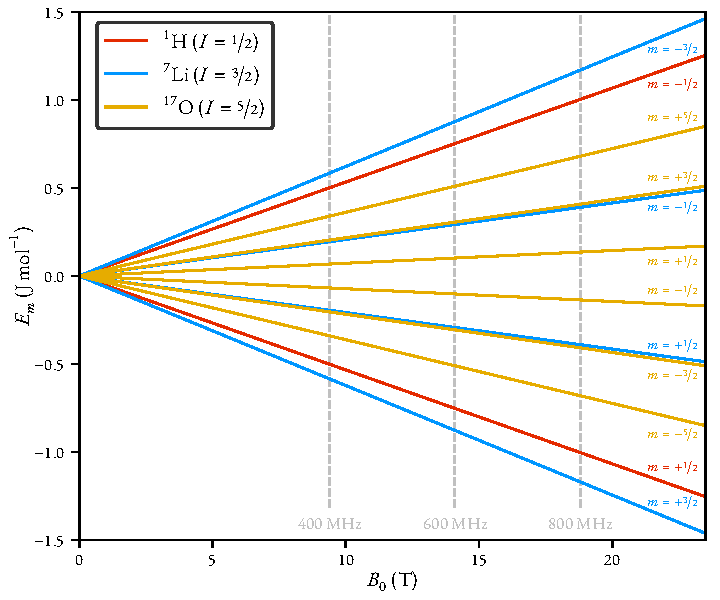
\includegraphics{energy_levels/energy_levels.pdf}
    \caption[
        The variation of energy of the spin states of \proton,
        \textsuperscript{7}Li, and \textsuperscript{17}O with external magnetic
        field strength.
    ]{
        The variation of energy of the spin states of \proton,
        \textsuperscript{7}Li, and \textsuperscript{17}O with external magnetic
        field strength ($B_0$), up to \qty{23.5}{\tesla}, which is
        approximately the strength of a \qty{1}{\giga \hertz} \ac{NMR} magnet.
        Three common field strengths for commercial NMR magnets are indicated:
        \qty{9.40}{\tesla} (\qty{400}{\mega\hertz}), \qty{14.10}{\tesla}
        (\qty{600}{\mega\hertz}), and \qty{18.79}{\tesla}
        (\qty{800}{\mega\hertz}).
    }
    \label{fig:energy_levels}
\end{figure}
\note{REVISIT THIS SECTION}
\ac{NMR} samples comprise a vast ensemble of equivalent spin systems, and it is
the macroscopic properties of the sample that are observed. Consider an
ensemble of $N$ spin-$I$ nuclei. At thermal equilibrium, the various spin
states will be disproportionately populated in accordance with the Boltzmann
distribution. Assuming that $\nicefrac{m \hbar \gamma B_0}{k_{\mathrm{B}}T} \gg
1$, which is the case for conventional temperatures, the proportion of spins in
state $m$ can be shown to be given approximately by\cite{Levitt2007}
\begin{equation}
  \frac{N_m}{N} \approx \frac{1}{2I + 1} \left( 1 + \frac{m \hbar \gamma B_0}{k_{\mathrm{B}} T} \right)
\end{equation}
where $k_{\mathrm{B}}$ is the Boltzmann constant. The ensemble has an
associated bulk magnetic moment $\symbf{M}$, given by the summation of all the
indivual spin magnetic moments:
\begin{equation}
  \symbf{M} = \gamma \symbf{J} = \sum\limits_{n=1}^N \symbf{\mu}_n
\end{equation}
where $\symbf{J}$ is the spin angular momentum of the ensemble. At equilibrium,
the $x$- and $y$-components of the bulk magnetisation are zero, i.e.
$\sum_{n=1}^N \mu_{x,n} = \sum_{n=1}^N \mu_{y,n} = 0$, such that magnetisation
is colinear with the field direction: $\symbf{M} = \left[0, 0, M_0
\right]^{\mathrm{T}}$, where $M_0$ is the magnitude of the bulk magnetism. The
time evolution of the angular momentum is equivalently the torque, which is
given by
\begin{equation}
  \symbf{\tau} = \frac{\mathrm{d}\symbf{J}(t)}{\mathrm{d}t} = \symbf{M}(t) \times \symbf{B}(t)
\end{equation}
Therefore, the rate of change of the bulk magnetism is
\begin{equation}
  \frac{\mathrm{d}\symbf{M}(t)}{\mathrm{d}t} = \symbf{M}(t) \times \gamma \symbf{B}(t),
\end{equation}
which results in the following expression under the assumption that
$\symbf{B}(t)$ is static and directed along the $z$-direction:

\subsection{The NMR Spectrometer}
A modern \ac{NMR} spectrometer has the capability of conducting a plethora of
experiments, thanks to the availability of high magnetic fields, sophisticated
electronics for pulse generation, and signal acquisition. An overview of the
key components of the spectrometer is presented here.

\subsubsection{The Magnet}
The resolution of \ac{NMR} data increases linearly with $B_0$, while sensitivity
increases as $B_0^{\nicefrac{3}{2}}$\cite{Abragam1961}, such that it is
desirable to use magnets that produce the highest fields
possible.\footnote{This relation isn't perfect, when features such as a
nucleus' chemical shift anisotropy are considered.} Conventional NMR magnets
feature a superconducing solenoid immersed in liquid He, which has a boiling
point of \qty{4.2}{\kelvin} at atmospheric pressure. Common materials used
for the solenoid include the type II superconductors Nb-Ti and
Nb\textsubscript{3}Sn. The dewar that the Helium is contained in is lined with
a thermal radiation shield, which is surrounded by a larger dewar of liquid
N\textsubscript{2}, to minimise the extent of He evaporation. Passing through
the magnet's $z$-direction is a bore, which is maintained at ambient
temperature, or some-other user specified temperature. Within this bore sits
the sample, as well as the probe.

To maintain high spatial field homogeneity - a necessity for results of
acceptable resolution - a series of coils called \textit{shims} surround the
sample. Each coil produces a weak magnetic field with a specific spatial
profile, which can cancel out any inhomogeneity inherent to the main magnet.

\subsubsection{The Probe}
The probe features the coil(s) used to pulse the sample with \ac{RF} radiation, as
well as recieve the resultant signal. A relatively recent development in probe
technology is the cryogenic probe\cite{Styles1984, Styles1989, Kovacs2005}. The
transmit/recieve coil(s) and other probe circuitury are maintained at very low
temperature ($\sim \num{25} \si{\kelvin}$), which reduces Johnson-Nyquist
noise. This manifests in a higher signal-to-noise ratio (SNR), which can be as
large as 4 times that achievable with conventional probes.

\subsubsection{The Transmitter}
The transmitter is the collection of components which generates \ac{RF} pulses. A
synthesiser acts as an \ac{RF} source, producing a continuous carrier wave at or
very close to the Larmor frequency. Pulses are subsequently produced by a
modulator, and are then amplitfied from a power of a few $\si{\milli \watt}$,
to $\si{\deca \watt}$, or even $\si{\hecto \watt}$\cite{Keeler2010}.

\subsubsection{The Reciever}

\subsubsection{The Pulse Programmer}

\subsection{The acquisition and structure of \acs{NMR} data}
In \ac{NMR} experiments, \ac{RF} pulses manipulate nuclear magnetic spin
states. While there is a plethora of different pulse sequences, the net effect
of all of them is the generation of magnetisation which is transverse to the
field direction. The evolution of this magnetisation induces a time-varying
electromotive force within the coil(s) of the probe, with the signal generated
being amplified and digitised by the receiver, generating \iac{FID}.
The \ac{FID} is sampled at equally-spaced time intervals $\Dt$, such that
it is of the form
\begin{equation}
  \symbf{y} =
  \begin{bmatrix}
      y(t=0) & y(t=\Dt) & y(t=2\Dt) & \cdots & y(t=(N-1)\Dt)
  \end{bmatrix}\T
\end{equation}
where $y(t)$ is the (continuous) variation of the generated signal with time,
and $N$ is the number of points sampled. The inverse of the sampling rate,
$\nicefrac{1}{\Dt}$ is the sweep width or spectral window $\fsw$ which
defines how wide the range of samplable frequencies is (see Appendix Section
\ref{sec:nyquist} for more on this).

\begin{figure}
    \centering
    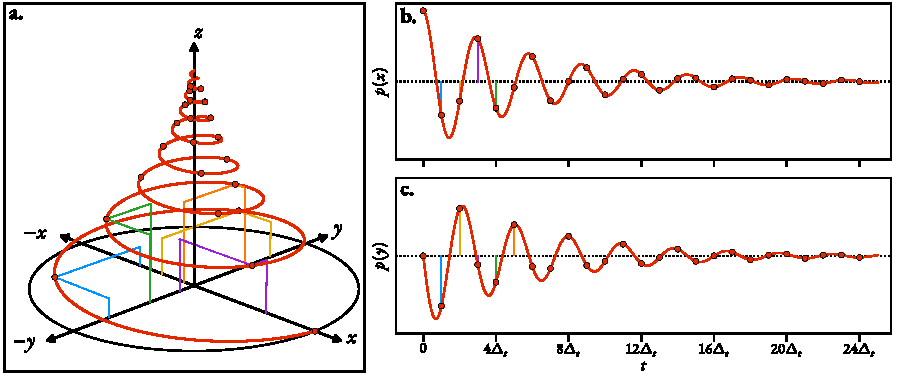
\includegraphics{quadrature_detection/quadrature_detection.pdf}
    \caption[
        An simple illustration of quadrature detection.
    ]{
        An illustration of quadrature detection using the vector
        model\cite[Chapter 1]{Hore2015}.
        \textbf{a.} An illustration of the evolution of the bulk magnetisation
        for a system comprising many identical spins, aligned initially along
        the laboratory $x$-axis (for example, immediately after a
        $\ang{90}_{-y}$ pulse in a pulse-acquire experiment). At regular time
        intervals separated by $\Dt$, the signal is sampled, such that the
        projection onto the $x$-axis, $p(x)$, and onto the $y$-axis, $p(y)$ is
        measured. For the first few samples, the projections onto the $x$- and
        $y$-axes are denoted by solid and dashed coloured lines, respectively.
        The complete projections are given in panels \textbf{b.} and
        \textbf{c.}. The \ac{FID} is given by the complex value $p(x) + \iu p(y)$.
    }\label{fig:quadrature}
\end{figure}

On modern spectrometers, a quadrature acquisition system is used\cite[Appendix
A.5]{Levitt2007} (see Figure \ref{fig:quadrature}), such that \acp{FID} adopt
the form of a summation of $M$ complex exponentials (oscillators), where $M \in
\mathbb{N}$ is the number of resonances contributing to the signal. Each
resonance will be subjected to damping due to relaxation phenomena, which is
typically exponential in nature.  An \ac{FID} acquired with $N$ samples $\by
\in \mathbb{C}^{N}$ therefore takes the form
\begin{subequations}
    \begin{gather}
        \by \left[n\right] =
            \bx \left[ n \right] +
            \bw \left[ n \right]
            \quad \forall n \in \lbrace 0, 1, \cdots, N - 1 \rbrace,
            \label{eq:y=x+w} \\
        \bx \left[n\right] =
            \sum_{m=0}^{M-1} \bdam \exp\left(
                \iu \bdphim
            \right) \exp\left(
                \left[ 2 \pi \iu \left(\bdfm - \foff\right)- \bdetam \right] n \Dt
            \right).
            \label{eq:x}
    \end{gather}
    \label{eq:1d}%
\end{subequations}%
$\foff$ is included to account for the transmitter offset, which is the
difference between the carrier wave frequency of the transmitter and the
spectrometer basic frequency. \eqref{eq:1d} indicates that \iac{FID} comprises
contributions from the (modellable) evolution of the spin magnetisation $\bx$
and experimental noise $\bw$ (\emph{vide infra}). Each oscillator which
contributes to $\bx$ is defined by four parameters:
\begin{itemize}
    \item $a \in \mathbb{R}_{>0}$ - the amplitude,
    \item $\phi \in (-\pi, \pi]$ - the phase,
    \item $f \in \left[\hspace*{2pt}\foff - \nicefrac{1}{2} \hspace*{2pt}
        \fsw, \foff + \nicefrac{1}{2} \hspace*{2pt}\fsw \right]$ - the frequency,
    \item $\eta \in \mathbb{R}_{>0}$ - the damping factor.
\end{itemize}%
\iac{FID} can therefore be parameterised by the vector $\bth \in
\mathbb{R}^{4M}$:
\begin{equation}
    \bth =
    \begin{bmatrix}
        \symbf{a}\T & \symbf{\phi}\T & \symbf{f}\T & \symbf{\eta}\T
    \end{bmatrix}\T,
\end{equation}
where $\bda \in \mathbb{R}^M$ is a vector of all amplitudes, $\bdphi \in
\mathbb{R}^M$ is a vector of all phases, etc.

Multidimensional experiments involve incrementing one or more experimental
parameters (a common example being a particular delay period in the pulse
sequence), in order to obtain an array of \ac{1D} \acp{FID}. In a $D$-dimensional
dataset, each contributing resonance is parameterised by an amplitude and phase
as before, and also $D$ distinct frequencies and corresponding damping factors,
such that a general parameter vector  $\bth \in \mathbb{R}^{2(1+D)M}$ is
given by
\begin{equation}
    \bth =
    \begin{bmatrix}
    \symbf{a}\T &
    \symbf{\phi}\T &
    \left[\symbf{f}^{(1)}\right]\T &
    \cdots &
    \left[\symbf{f}^{(D)}\right]\T &
    \left[\symbf{\eta}^{(1)}\right]\T &
    \cdots &
    \left[\symbf{\eta}^{(D)}\right]\T
    \end{bmatrix}\T,
\end{equation}
where $\bdfD$ and $\bdetaD$ are the frequencies and damping factors in the
actively acquired (direct) dimension, and $\bdfone$ -- $\bdfDminusone$ and
$\bdetaone$ -- $\bdetaDminusone$ are those for the indirect dimension(s).
Indirect dimensions can exhibit different forms of evolution, depending on
the precise nature of the pulse sequence. Two common functional
forms exist\cite[Section 4.3.4]{Cavanagh2007}. Signals of the form $\cos(2 \pi
f t)$ and $\sin(2 \pi f t)$ modulate the amplitude of the direct
dimension signal across increments, while those of the form $\exp(2 \pi \iu f
t)$ or $\exp(-2 \pi \iu f t)$ modulate the phase.  Amplitude- or
phase-modulated signals are often acquired as pairs when possible, as this
ensures that frequency-discriminated spectra can be generated with
absorption-mode Lorentzian lineshapes in all dimensions (\emph{vide infra}). In
general, a $D$-dimensional \ac{FID}
$\bY \in \mathbb{C}^{\None \times \cdots \times \ND}$ can be expressed as
\begin{subequations}
    \begin{gather}
        \begin{split}
            \bY\left[\none, \cdots, \nD\right] =
                &\sum_{m=0}^{M-1} \bdam \exp\left( \iu \bdphim \right) \\
                &\times \prod_{d=1}^D
                \zeta\left(2 \pi \left(\symbf{f}^{(d)}_{\vphantom{\text{off}}}[m]  - \foffd\right) \nd \Dtd\right)
                \exp\left(-\symbf{\eta}^{(d)}_{\vphantom{\text{off}}}[m] \nd \Dtd\right)\\
                &+\symbf{W}\left[n^{(1)}, \cdots, n^{(D)}\right]
        \end{split}\\
        \zeta(\cdot)
        \begin{cases}
            = \exp(\iu\cdot) & d = D \\
            \in \left\lbrace \cos(\cdot), \sin(\cdot), \exp(\iu\cdot) \exp(-\iu\cdot)\right\rbrace & \text{otherwise}
        \end{cases},
    \end{gather}
    \label{eq:general-fid}%
\end{subequations}%

Without any specific knowledge about the experiment, it is typical to assume
that $\symbf{W}$ is an array of \ac{AWGN}, meaning that the noise instances
are described by a complex normal distribution with mean 0, and
pairs of noise instances are statistically independent, regardless of their
time separation:
\begin{equation}
    \begin{gathered}
        \symbf{W}\left[n^{(1)}, \cdots, n^{(D)}\right] \coloneq w \sim
        \mathcal{N_C}\left(0, 2\sigma^2\right) \\
        \implies \Re\left(w\right) \upmodels \Im\left(w\right),
             \Re\left(w\right) \sim \mathcal{N}\left(0, \sigma^2\right),
             \Im\left(w\right) \sim \mathcal{N}\left(0, \sigma^2\right). \\
    \end{gathered}
\end{equation}
\note{Double check the equations are right for the SNR below...}{
The extent by which a signal is corrupted by noise is given by the \ac{SNR},
the ratio of signal power and noise power: \note{definition of power in
appendix}
\begin{equation}
    \begin{split}
        \SNR\left(\bY\right) &\coloneq \frac{P_{\bX}}{P_{\bW}}, \\
        &=\frac{1}{2 \mathfrak{N} \sigma^2}
            \sum_{\none=0}^{\None-1} \cdots \sum_{\nd=0}^{\ND-1}
            \left \lvert \bX \left[\none, \cdots, \nD \right] \right \rvert^2,
    \end{split}
\end{equation}
where $\mathfrak{N} \coloneq \None \cdots \ND$ is the total number of points
the signal comprises. Due to the large dynamic range that the \ac{SNR} can
exhibit, it is common to express it using a logarithmic scale instead,
in units of decibels (\unit{\deci\bel}):
\begin{equation}
    \begin{split}
        \SNR_{\unit{\deci\bel}} &\coloneq 10 \log_{10} \left(\SNR\right).
    \end{split}
\end{equation}
From this, the noise variance associated with a signal whose noiseless component is $\bX$ is given by
\begin{equation}
    \sigma^2 = \frac{1}{ 20^{\frac{\SNR_{\unit{\deci\bel}}}{10}}\mathfrak{N}}
        \sum_{\none=0}^{\None-1} \cdots \sum_{\nd=0}^{\ND-1}
        \left \lvert \bX \left[\none, \cdots, \nD \right] \right \rvert^2.
\end{equation}
